\documentclass{article}
\usepackage[widepage]{repsty}

\usepackage[utf8]{inputenc}
\usepackage[T1]{fontenc}
\usepackage[english, russian]{babel}

\newcommand{\MDM}{^\mathrm{MDM}}
\newcommand{\EDM}{^\mathrm{EDM}}
\newcommand{\EMDM}{^\mathrm{E+M}}
\newcommand{\pauli}{\vec{\sigma}}

\begin{document}

Еремей, привет!

Я хотел бы узнать твоё мнение по поводу того, как я симулирую процедуру калибровки.
Сначала несколько вводных утверждений:
\begin{enumerate}
	\item Я хочу вычислить spin tune \& invariant spin axis;
	\item для этого правильнее всего использовать: TSS MU NBAR 0, но при выполнении FS условия у меня возникает спин-орбитальный резонанс, и MU, NBAR не вычисляются;
	\item Артём предложил, чтобы уйти от резонанса, просто добавить EDM в симуляцию: из-за $EDM \neq 0$ я должен отойти от резонансной точки, и тогда проблемы в TSS не возникнет.
\end{enumerate}	

Для того, чтобы симулировать EDM, я использую процедуру RSX. Как я это делаю представлено на рис.~\ref{fig:script}, сама процедура на рис.~\ref{fig:rsx}.
	\begin{figure}[h]
		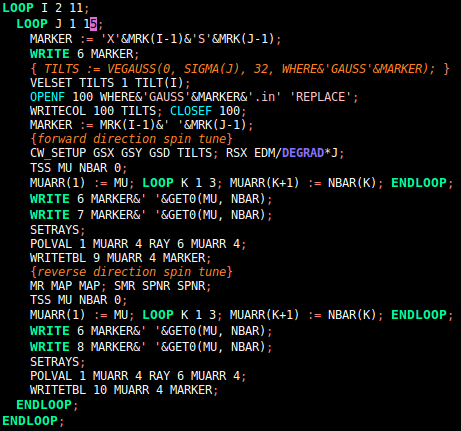
\includegraphics{CALIB_DANF_SCRIPT}
		\caption{Тестовый скрипт для моделирования калибровки\label{fig:script}}
	\end{figure}
	\begin{figure}[h]
		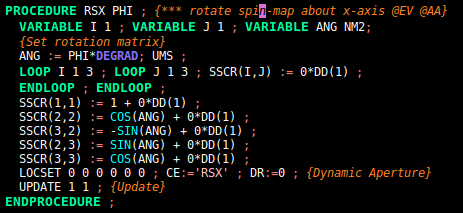
\includegraphics{RSX_procedure}
		\caption{Процедура для симулирования эффекта от EDM.\label{fig:rsx}}
	\end{figure}
	
Процедура CW\_SETUP это просто последовательность элементов; я убрал её (последовательность) в отдельный фаил, в эту процедуру, чтобы импортировать в скрипты для разных симуляций.

Как я понимаю, скрипт из рис.~\ref{fig:script} делает следующее:
\begin{enumerate}
	\item Сначала CW\_SETUP вычисляет SPNR, что математически можно записать как $e\MDM \equiv \exp\bkt*{\imath\cdot \nu_s\MDM(\hat n \cdot \pauli)}$;
	\item После этого RSX делает преобразование $e\EMDM \equiv \underbrace{\exp\bkt*{\imath\cdot \nu_s\EDM(\hat x \cdot \pauli)}}_{SSRC} \underbrace{e\MDM}_{SPNR}$.
	\item После этого я вычисляю полиномы MU, NBAR для $e\EMDM$;
	\item Затем я вычисляю значения этих полиномов на лучах, вывожу это для дальнейшей обработки.
	\item После этого SMR вычисляет обратный элемент $e\EMDM_{rev} \equiv \bkt{e\EMDM}^{-1}$, и я повторяю процедуру.
\end{enumerate}

В результате, для частицы на замкнутой орбите ($Z = (0,0,0,0,0,0)$) я получаю:
\begin{itemize}
	\item $MU|0^{FWD} = MU|0^{REV}$,
	\item $NBAR(1)|0^{FWD} = NBAR(1)|0^{REV} \approx -1$,
	\item $NBAR(2)|0^{FWD} = NBAR(2)|0^{REV} \approx 1.5e-3$,
	\item $NBAR(3)|0^{FWD} = - NBAR(3)|0^{REV} \approx -2.4e-2$.
\end{itemize} 

Я работаю на энергии 234.6266 МэВ; это около Frozen Spin энергии.
\end{document}